\documentclass{unswmaths}
\usepackage{unswshortcuts}
\usepackage{hyperref}
\usepackage{ dsfont }
\begin{document}
\author{Adam J. Gray}
\title{Assignment 3}
\subject{Ergodic Theory}
\studentno{3329798}

\unswtitle

\section{}
    We consider the map
    \begin{align}
        T(x) = 
        \begin{cases}
            2x + \frac{1}{2} & 0 \leq x < \frac{1}{4} \\
            -x + \frac{5}{4} & \frac{1}{4} \leq x < \frac{1}{2} \\
            -2x + \frac{7}{4} & \frac{1}{2} \leq x < \frac{3}{4} \\
            -x + 1 & \frac{3}{4} \leq x \leq 1.
        \end{cases}
    \end{align}
    This has the following plot:
    
    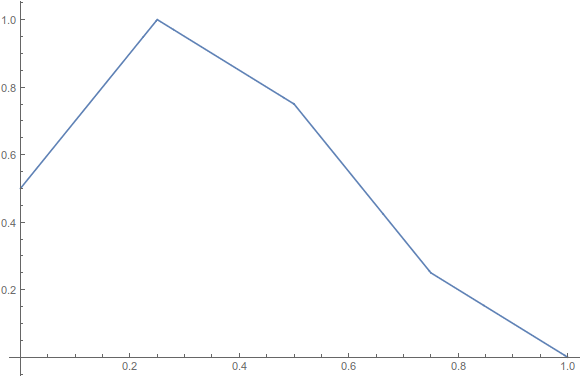
\includegraphics[scale=0.5]{qn_1_map}
\subsection{}
    We have that in general
    \begin{align}
        \mathcal{P}_T f(x) = \sum_{z \in T^{-1} x} \frac{f(z)}{|T'(z)|}.
    \end{align}
    Then in general we have
    \begin{align}
        T'(x) = 
        \begin{cases}
            2 & 0 \leq x < \frac{1}{4} \\
            -1 & \frac{1}{4} \leq x < \frac{1}{2} \\
            -2 & \frac{1}{2} \leq x < \frac{3}{4} \\
            -1 & \frac{3}{4} \leq x \leq 1.
        \end{cases}    
    \end{align}
    Also we can also see that
    \begin{align}
        T^{-1}\{x\} =
        \begin{cases}
            \{1-x\} & 0 \leq x < \frac{1}{4} \\
            \{\frac{7}{8} - \frac{x}{2} \} & \frac{1}{4} \leq x < \frac{1}{2} \\
            \{\frac{7}{8} - \frac{x}{2} \} \cup \{\frac{x}{2} - \frac{1}{4}\} & \frac{1}{2} \leq x < \frac{3}{4} \\
            \{\frac{5}{4} - x\} \cup \{ \frac{x}{2} - \frac{1}{4} \} & \frac{3}{4} \leq x < 1
        \end{cases}
    \end{align}
    thus for $ f_i(x) = \mathds{1}_{I_i}(x) $
    we have that
    \begin{align}
        \mathcal{P}_T f_1(x) &= \mathds{1}_{(\frac{3}{4},1)}(x) \\
        \mathcal{P}_T f_2(x) &= \mathds{1}_{(\frac{5}{8},\frac{3}{4})}(x) \\
        \mathcal{P}_T f_3(x) &= \frac{1}{2}\mathds{1}_{(\frac{1}{2},\frac{5}{8})}(x) + \frac{1}{2}\mathds{1}_{(0,\frac{1}{8})}(x) \\
        \mathcal{P}_T f_4(x) &= \frac{1}{2}\mathds{1}_{(\frac{1}{8},\frac{1}{4})}(x) + \mathds{1}_{(\frac{1}{4},\frac{1}{2})}(x) \\
    \end{align}
\section{}
\section{}
\section{}
\end{document}
